\documentclass[a4paper,12pt,fleqn]{article}

\usepackage{amsmath,amssymb,amsthm}
\usepackage[margin=1in]{geometry}
\usepackage{xcolor}
%\usepackage{url}
%\usepackage{float}
%\usepackage{array}
\usepackage{comment}
\usepackage{tikz}
\usetikzlibrary{arrows.meta}
\usepackage{tabularray}
%\usepackage{enumitem}
\usepackage[hypertexnames=false,bookmarksnumbered=true,final]{hyperref}
%\usepackage{algorithm,algpseudocode}
\usepackage[capitalize,sort]{cleveref}

\def\colorschemesepia{sepia}
\def\colorschemedark{dark}
\def\colorschemelight{light}

\ifx\colorscheme\undefined
\let\colorscheme\colorschemelight
\fi

\ifx\colorscheme\colorschemelight
\colorlet{textColor}{black}
\colorlet{bgColor}{white}
\fi

\ifx\colorscheme\colorschemesepia
\definecolor{textColor}{HTML}{433423}
\definecolor{bgColor}{HTML}{fbf0da}
\fi

\ifx\colorscheme\colorschemedark
\definecolor{textColor}{HTML}{bdc1c6}
\definecolor{bgColor}{HTML}{202124}
\definecolor{textBlue}{HTML}{8ab4f8}
\definecolor{textRed}{HTML}{f9968b}
\colorlet{bgRed}{red!40!black}
\colorlet{bgBlue}{red!40!black}
\else
\colorlet{textBlue}{blue!50!black}
\colorlet{textRed}{red!50!black}
\fi

\ifx\colorscheme\colorschemelight\else
\pagecolor{bgColor}
\color{textColor}
\fi

\hypersetup{colorlinks,linkcolor=textRed,citecolor=textRed,urlcolor=textBlue}

% THEOREMS

\newtheorem{theorem}{Theorem}
\newtheorem{definition}{Definition}
\newtheorem{example}{Example}
\newtheorem{corollary}{Corollary}[theorem]
\newtheorem{lemma}[theorem]{Lemma}
\newtheorem{claim}[theorem]{Claim}

% SHORTHANDS

\newcommand*{\Th}{^{\textrm{th}}}
\newcommand*{\WLoG}{Without loss of generality}
\newcommand*{\wLoG}{without loss of generality}
\newcommand*{\wrt}{with respect to}
\let\opname\operatorname

% SYMBOLS

\let\eps\epsilon
\newcommand*{\defeq}{:=}

\newcommand*{\alphahat}{\widehat{\alpha}}
\newcommand*{\betahat}{\widehat{\beta}}
\newcommand*{\Ahat}{\widehat{A}}
\newcommand*{\Bhat}{\widehat{B}}
\newcommand*{\Chat}{\widehat{C}}
\newcommand*{\Jhat}{\widehat{J}}
\newcommand*{\Shat}{\widehat{S}}
\newcommand*{\Yhat}{\widehat{Y}}
\newcommand*{\bhat}{\widehat{b}}
\newcommand*{\shat}{\widehat{s}}
\newcommand*{\what}{\widehat{w}}
\newcommand*{\xhat}{\widehat{x}}
\newcommand*{\yhat}{\widehat{y}}
\newcommand*{\zhat}{\widehat{z}}

\newcommand*{\Btild}{\widetilde{B}}
\newcommand*{\Ctild}{\widetilde{C}}
\newcommand*{\Jtild}{\widetilde{J}}
\newcommand*{\Stild}{\widetilde{S}}
\newcommand*{\Ytild}{\widetilde{Y}}
\newcommand*{\btild}{\widetilde{b}}
\newcommand*{\stild}{\widetilde{s}}
\newcommand*{\wtild}{\widetilde{w}}
\newcommand*{\xtild}{\widetilde{x}}
\newcommand*{\ytild}{\widetilde{y}}
\newcommand*{\ztild}{\widetilde{z}}

\newcommand*{\Fcal}{\mathcal{F}}
\newcommand*{\Tcal}{\mathcal{T}}

\newcommand*{\ebar}{\overline{e}}
\newcommand*{\Xbar}{\overline{X}}
\newcommand*{\xbar}{\overline{x}}
\newcommand*{\Ybar}{\overline{Y}}
\newcommand*{\ybar}{\overline{y}}

% MATH

\newcommand*{\floor}[1]{\left\lfloor #1 \right\rfloor}
\newcommand*{\smallfloor}[1]{\lfloor #1 \rfloor}
\newcommand*{\ceil}[1]{\left\lceil #1 \right\rceil}
\newcommand*{\smallceil}[1]{\lceil #1 \rceil}
\newcommand*{\abs}[1]{\left\lvert #1 \right\rvert}
\newcommand*{\smallabs}[1]{\lvert #1 \rvert}
\newcommand*{\norm}[1]{\left\lVert #1 \right\rVert}
\newcommand*{\smallnorm}[1]{\lVert #1 \rVert}
\newcommand*{\Z}{\mathbb{Z}}
\DeclareMathOperator*{\E}{E}
\DeclareMathOperator*{\Var}{Var}
\DeclareMathOperator*{\argmin}{argmin}
\DeclareMathOperator*{\argmax}{argmax}
\DeclareMathOperator{\poly}{poly}
\DeclareMathOperator{\opt}{opt}
\DeclareMathOperator{\argopt}{argopt}
\DeclareMathOperator{\support}{support}
\newcommand*{\OPT}{\mathrm{OPT}}


%\def\checkmark{\tikz\fill[scale=0.4](0,.35) -- (.25,0) -- (1,.7) -- (.25,.15) -- cycle;}

\allowdisplaybreaks
%\algnewcommand{\LineComment}[1]{\State \textcolor{gray}{\texttt{//} \textit{#1}}}
%\renewcommand{\algorithmiccomment}[1]{\hfill\textcolor{gray}{\texttt{//} \textit{#1}}}

\title{Bipartite Matching}
\author{Eklavya Sharma}
\date{\empty}

\begin{document}

\maketitle
\setlength{\parindent}{0pt}
\setlength{\parskip}{0.5em}

\begin{abstract}
This document describes an algorithm for perfect matching in bipartite graphs
and the Hungarian Algorithm for min-cost perfect matching.
Full proofs are not given, but the high-level idea is conveyed,
so that it's intuitively clear what's going on in the algorithms.
\end{abstract}

\section{Bipartite Graphs and Perfect Matching}

Let $G = (L \cup R, E)$ be a bipartite graph, where $L$ is the set of left vertices,
$R$ is the set of right vertices, and $E \subseteq L \times R$ is the set of edges.
A subset $M \subseteq E$ of edges is called a \emph{matching} in $G$
if no two edges of $M$ share an endpoint.
If $M$ is a matching and $|L| = |R| = |M|$, then $M$ is called a \emph{perfect matching}.
See \cref{fig:ex-pmatch} for an example.

\begin{figure}[htb]
\centering
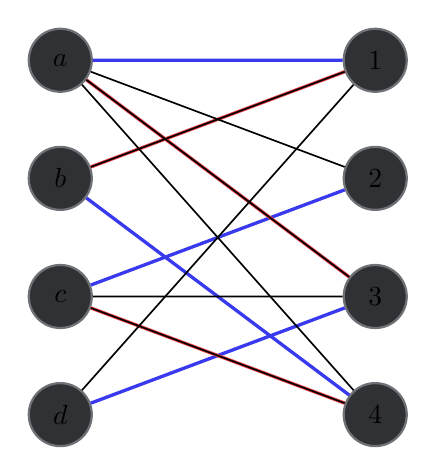
\begin{tikzpicture}[
vertex/.style={shape=circle,draw={textColor!50!bgColor},fill={textColor!10!bgColor},thick,
    minimum size=8mm,inner sep=0},
%myarrow/.style={->,>={Stealth},semithick},
myedge/.style={semithick},
blueEdge/.style={very thick,draw={blue!70!textColor}},
redEdge/.style={very thick,draw={red!70!textColor}}
]
\node[vertex] (l1) at (0,4.5) {$a$};
\node[vertex] (l2) at (0,3.0) {$b$};
\node[vertex] (l3) at (0,1.5) {$c$};
\node[vertex] (l4) at (0,0.0) {$d$};
\node[vertex] (r1) at (4,4.5) {$1$};
\node[vertex] (r2) at (4,3.0) {$2$};
\node[vertex] (r3) at (4,1.5) {$3$};
\node[vertex] (r4) at (4,0.0) {$4$};
\draw[blueEdge] (l1) -- (r1) (l2) -- (r4) (l3) -- (r2) (l4) -- (r3);
\draw[redEdge] (l1) -- (r3) (l2) -- (r1) (l3) -- (r4);
\draw[myedge] (l1) -- (r2) (l1) -- (r3) (l1) -- (r4);
\draw[myedge] (l2) -- (r1);
\draw[myedge] (l3) -- (r3) (l3) -- (r4);
\draw[myedge] (l4) -- (r1);
\end{tikzpicture}
\caption{A bipartite graph. The blue edges form a perfect matching.
The red edges form an imperfect matching.}
\label{fig:ex-pmatch}
\end{figure}

\begin{table}[htb]
\centering
\caption{Graph of \cref{fig:ex-pmatch} in tabular format.}
\label{table:ex-pmatch}
\begin{tblr}{
colspec={|c|[1.2pt]c|c|c|c|},
rowspec={|Q|[1.2pt]Q|Q|Q|Q|},
cell{2}{2}={bg={blue!10!bgColor},fg=textBlue},
cell{3}{5}={bg={blue!10!bgColor},fg=textBlue},
cell{4}{3}={bg={blue!10!bgColor},fg=textBlue},
cell{5}{4}={bg={blue!10!bgColor},fg=textBlue},
cell{2}{4}={bg={red!10!bgColor},fg=textRed},
cell{3}{2}={bg={red!10!bgColor},fg=textRed},
cell{4}{5}={bg={red!10!bgColor},fg=textRed},
}
 & 1 & 2 & 3 & 4
\\ $a$ & \checkmark & \checkmark & \checkmark & \checkmark
\\ $b$ & \checkmark & $\times$   & $\times$   & \checkmark
\\ $c$ & $\times$   & \checkmark & \checkmark & \checkmark
\\ $d$ & \checkmark & $\times$   & \checkmark & $\times$
\end{tblr}
\end{table}

We can also represent bipartite graphs as a table.
Each row of the table represents a left vertex
and each column represents a right vertex.
The cell $(u, v)$ contains \checkmark{} if an edge exists from $u$ to $v$ and $\times$ otherwise.
See \cref{table:ex-pmatch} for an example.
A subset of edges forms a matching if for any two edges in that subset,
their cells have different rows and different columns.

Here we will focus on two problems:
\begin{enumerate}
\item \emph{Maximum cardinality matching}:
    Given a bipartite graph, find a matching $M$ such that $|M|$ is maximized.
\item \emph{Min-cost perfect matching}:
    Given a bipartite graph, and given the cost of edge edge,
    find a minimum-cost perfect matching, or report that no perfect matching exists.
\end{enumerate}

\section{Primal-Dual Technique}

Sometimes, it's hard to solve a problem but easy to verify the solution.
E.g., in the factoring problem, we are given a large natural non-prime number $x$,
and we need to output two natural numbers $y$ and $z$ larger than 1 such that $x = yz$.
Factoring the number $x = 2252989$ by hand is quite time-consuming.
But if I tell you that the factors are $y = 1117$ and $z = 2017$, it's easy to verify that they
are indeed the factors by simply multiplying these numbers to compute $yz$
and then checking that $x$ equals $yz$.
Similarly, solving a sudoku puzzle is not easy, but verifying a solution is simple:
just check that each row, column, and $3\times3$ box is a permutation of $\{1, 2, \ldots, 9\}$.

The ability to easily verify solutions to a problem can make life much easier.
Imagine spending a lot of time trying to solve a problem,
and having no way of easily checking whether you got the right answer.
That would be bad, right?
Also, verifiability helps us use \emph{hit-and-trial} to solve the problem,
i.e., repeatedly guess a solution and check if it's a correct solution.

For some problems, it's not obvious how to verify the solution.
E.g., for linear programming, given a vector $x$, it's not obvious how to easily check
whether $x$ is an optimal solution to the LP.
We can find the optimal objective value of the LP (e.g., using the simplex method)
and then compare that to $x$'s objective value to check whether $x$ is optimal,
but that would be very time-consuming.

However, suppose we want to solve both the primal and the dual LPs.
Given two vectors $x$ and $y$, it is easy to check whether they are optimal solutions
to the primal and dual LPs, respectively, using the strong duality of linear programs:
just check that $x$ is feasible for the primal, $y$ is feasible for the dual,
and that $x$ and $y$ have the same objective value.

This technique of solving problems by simultaneously finding a primal and dual solution
is called the \emph{primal-dual technique}.
We will use this technique in the algorithms in this document.

\section{Maximum Cardinality Matching}

\subsection{Hit-and-Trial}

\begin{definition}
In a bipartite graph $G = (L \cup R, E)$, a set $S \subseteq L \cup R$ of vertices
is a vertex cover if for every edge in $E$, at least one of its endpoints is in $S$.
\end{definition}

In the minimum cardinality vertex cover problem, we are given a bipartite graph
and we need to find a vertex cover $S$ such that $|S|$ is minimum.
We can use linear programming duality to show that this problem is the dual of max cardinality matching.
Hence, if $M$ is a matching and $S$ is a vertex cover, then $|M| \le |S|$.
Although this can be proved using weak LP duality, we will give a direct proof of this fact:

\begin{lemma}[weak duality: matching vs vertex cover]
Let $G = (L \cup R, E)$ be a bipartite graph.
Let $M \subseteq E$ be a matching and $S \subseteq L \cup R$ be a vertex cover.
Then $|M| \le |L|$.
\end{lemma}
\begin{proof}
For each edge in $M$, at least one of its endpoints lies in $S$.
Since edges of $M$ don't share endpoints (because it's a matching),
we get that there must be at least $|M|$ vertices in $S$.
\end{proof}

Therefore, if we can find a matching $M$ and a vertex cover $S$ such that $|M| = |S|$,
then $M$ is a maximum cardinality matching (and $S$ is a min vertex cover).
See \cref{fig:ex-mcmatch}.

\begin{figure}[htb]
\centering
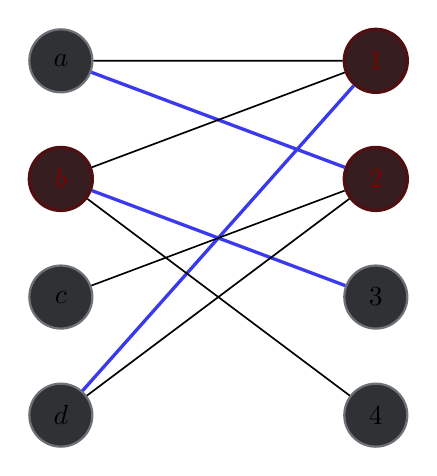
\begin{tikzpicture}[
vertex/.style={shape=circle,draw={textColor!50!bgColor},fill={textColor!10!bgColor},thick,
    minimum size=8mm,inner sep=0},
cVertex/.style={shape=circle,draw={textRed!50!bgColor},fill={red!10!bgColor},very thick,
    minimum size=8mm,inner sep=0},
%myarrow/.style={->,>={Stealth},semithick},
myedge/.style={semithick},
blueEdge/.style={very thick,draw={blue!70!textColor}}
]
\node[vertex] (l1) at (0,4.5) {$a$};
\node[cVertex] (l2) at (0,3.0) {\textcolor{textRed}{$b$}};
\node[vertex] (l3) at (0,1.5) {$c$};
\node[vertex] (l4) at (0,0.0) {$d$};
\node[cVertex] (r1) at (4,4.5) {\textcolor{textRed}{$1$}};
\node[cVertex] (r2) at (4,3.0) {\textcolor{textRed}{$2$}};
\node[vertex] (r3) at (4,1.5) {$3$};
\node[vertex] (r4) at (4,0.0) {$4$};
\draw[blueEdge] (l1) -- (r2) (l2) -- (r3) (l4) -- (r1);
\draw[myedge] (l1) -- (r1) (l2) -- (r1) (l2) -- (r4) (l3) -- (r2) (l4) -- (r2);
\end{tikzpicture}
\caption{Blue edges give us a matching \textcolor{textBlue}{$M$}.
Red vertices give us a vertex cover \textcolor{textRed}{$S$}.
We know that $M$ is a maximum cardinality matching in this graph since $|M| = |S|$.}
\begin{tblr}{
colspec={|c|[1.2pt]c|c|c|c|},
rowspec={|Q|[1.2pt]Q|Q|Q|Q|},
cell{2}{3}={bg={blue!10!bgColor},fg=textBlue},
cell{3}{4}={bg={blue!10!bgColor},fg=textBlue},
cell{5}{2}={bg={blue!10!bgColor},fg=textBlue},
cell{1}{2,3}={bg={red!10!bgColor},fg=textRed},
cell{3}{1}={bg={red!10!bgColor},fg=textRed},
}
 & 1 & 2 & 3 & 4
\\ $a$ & \checkmark & \checkmark & $\times$ & $\times$
\\ $b$ & \checkmark & $\times$   & \checkmark & \checkmark
\\ $c$ & $\times$   & \checkmark & $\times$ & $\times$
\\ $d$ & \checkmark & \checkmark & $\times$ & $\times$
\end{tblr}
\label{fig:ex-mcmatch}
\end{figure}

Furthermore, this approach is guaranteed to work, i.e.,
if $M$ is a maximum cardinality matching and $S$ is a minimum vertex cover, then $|M| = |S|$.
We cannot prove this using strong LP duality alone.
We would also need to prove that optimal solutions are integral.
We can prove it using the max-flow min-cut theorem
(the proof is beyond the scope of this document).

\subsection{Augmenting Path Algorithm}

(TODO)

\section{Min-Cost Perfect Matching}

(TODO)

%\bibliographystyle{plainurl}
%\bibliography{bibdb}

\end{document}
